%20 min preso!
\documentclass[xcolor=table,english]{beamer}
\usepackage{beamerthemesplit}
\usepackage{wrapfig}
\usetheme{SPbGU}
\usepackage{pdfpages}
\usepackage{amsmath}
\usepackage{mathtools}
\usepackage{cmap}
\usepackage{subcaption}
\usepackage[utf8]{inputenc}
\usepackage[T1, T2A]{fontenc}
\usepackage[]{babel}
\usepackage{indentfirst}
\usepackage{amsmath}
\usepackage{tikz}
\usepackage{multirow}
\usepackage[noend]{algpseudocode}
\usepackage{algorithm}
\usepackage{algorithmicx}
\usepackage{fancyvrb}
\usetikzlibrary{calc}
\usetikzlibrary{shapes,arrows}
\usetikzlibrary{arrows,automata}
\usetikzlibrary{positioning}
\usetikzlibrary{fit}

\usepackage{kbordermatrix} % include package @ document preamble
\renewcommand{\kbldelim}{(} % change default array delimiters to parentheses
\renewcommand{\kbrdelim}{)}

\newcommand\mca{\multicolumn{1}{c}{\cellcolor{red}\textbf{\{a\}}}}
\newcommand\mcb{\multicolumn{1}{c}{\cellcolor{red}\textbf{\{b\}}}}

\usepackage{tabularx}
\newcolumntype{Y}{>{\raggedleft\arraybackslash}X}

\renewcommand{\thealgorithm}{}

\newtheorem{mytheorem}{Theorem}
\renewcommand{\thealgorithm}{}

\newcommand{\tikzmark}[1]{\tikz[overlay,remember picture] \node (#1) {};}
\def\Put(#1,#2)#3{\leavevmode\makebox(0,0){\put(#1,#2){#3}}}

\newcommand{\ltz}{$< 1$}


\tikzset{
    state/.style={
           rectangle,
           rounded corners,
           draw=black, very thick,
           minimum height=2em,
           inner sep=2pt,
           text centered,
           },
}

\beamertemplatenavigationsymbolsempty

\title[Dynamic Graphs GPU]{Dynamic Graphs on the GPU}
% \subtitle[YaccConstructor]{Parsing techniques for graph analysis}
% То, что в квадратных скобках, отображается в левом нижнем углу.
\institute[СПбГУ]{
JetBrains Research, Лаборатория языковых инструментов  \\
Санкт-Петербургский Государственный университет
}

% То, что в квадратных скобках, отображается в левом нижнем углу (прикольно).
\author[Егор Орачев]{\textbf{Егор Орачев}}

\date{2 Октября 2020}


\begin{document}
{
\begin{frame}[fragile]
  \begin{table}
  \centering
  \begin{tabularx}{\linewidth}{YcX}
    
\includegraphics[height=1.5cm]{pictures/jetbrainsResearch.pdf} \hfill
    & \begin{minipage}[t]{0.3\textwidth}\center \vspace{-1cm}  Семинар
      \end{minipage}
    & \hfill 
\includegraphics[height=1.5cm]{pictures/SPbGU_Logo.png}
  \end{tabularx}
  \end{table}
  \titlepage
\end{frame}
}

\begin{frame}[fragile] \frametitle{Мотивация} 
    \begin{minipage}[m]{0.45\linewidth}
        \begin{figure}
            \centering
            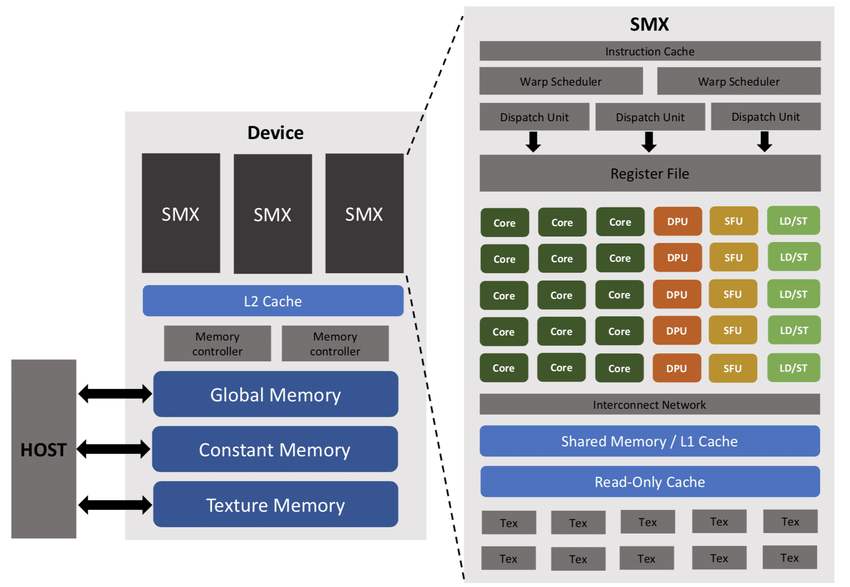
\includegraphics[width=\textwidth]{pictures/gpu_architecture.png}
            \caption{Generic GPU Architecture}
            \label{fig:architecture}
        \end{figure}
    \end{minipage}\hfill
    \begin{minipage}[m]{0.55\linewidth}
        \begin{itemize}
            \item Развитие GPU как платформы для вычислений
            \item Увеличение количества обрабатываемых данных
            \item Все больше и больше вычислительно сложных операций переходят на GPU 
                  (особенно, если мы хотим оставаться в пределах одного кластера)
        \end{itemize}
    \end{minipage}
\end{frame}

\begin{frame}[fragile] \frametitle{Идея}
    \begin{itemize}
        \item На данный момент большинство алгоритмов обработки графов на GPU 
              предполагают неизменяемость данных
        \item Большинство вычислений выглядят как: загрузить в VRAM, посчитать, 
              выгрузить обратно в RAM
        \item Вопрос: можно ли поддерживать структура графа в VRAM, и осуществлять доступ 
              к ней посредством операций, которые будут выполняться на GPU
    \end{itemize}
\end{frame}

\begin{frame}[fragile] \frametitle{Динамические графы на GPU} 
    \begin{itemize}
        \item В свежей статье\footnote{Dynamic Graphs on the GPU, Muhammad A. Awad, 
              Saman Ashkiani, Serban D. Porumbescu et al., ссылка: 
              \href{https://escholarship.org/uc/item/48j4k7np}{https://escholarship.org/uc/item/48j4k7np}} 
              приведены результаты, показывающие, что теоретически возможно поддерживать граф на GPU
        \item Цель: поддерживать \textit{истинно} динамические сценарии обновления, т.е. непрерывное             добавление, удаление вершин и ребер, а также высокую скорость поиска ребер
        \item Допущения: $|E| \ll |V|^2$
        \item Реализация: CUDA C
    \end{itemize}
\end{frame}

\begin{frame}[fragile] \frametitle{Структура графа}
    \begin{itemize}
        \item Граф: $G = (V,E,W)$
        \item Ребро графа: $e = (u,v,w)$
        \item Все ребра $e = (u,v,*)$ уникальны
        \item Ребра индексируются \textit{uint32}: до 4294967296 вершин 
        \item Веса индексируются \textit{uint32}: до 4294967296 уникальных весов
        \item Специальное значение $\perp$ для пустых ячеек
    \end{itemize}
\end{frame}

\begin{frame}[fragile] \frametitle{Структура графа}
    \begin{minipage}[m]{0.95\linewidth}
        \begin{figure}
            \centering
            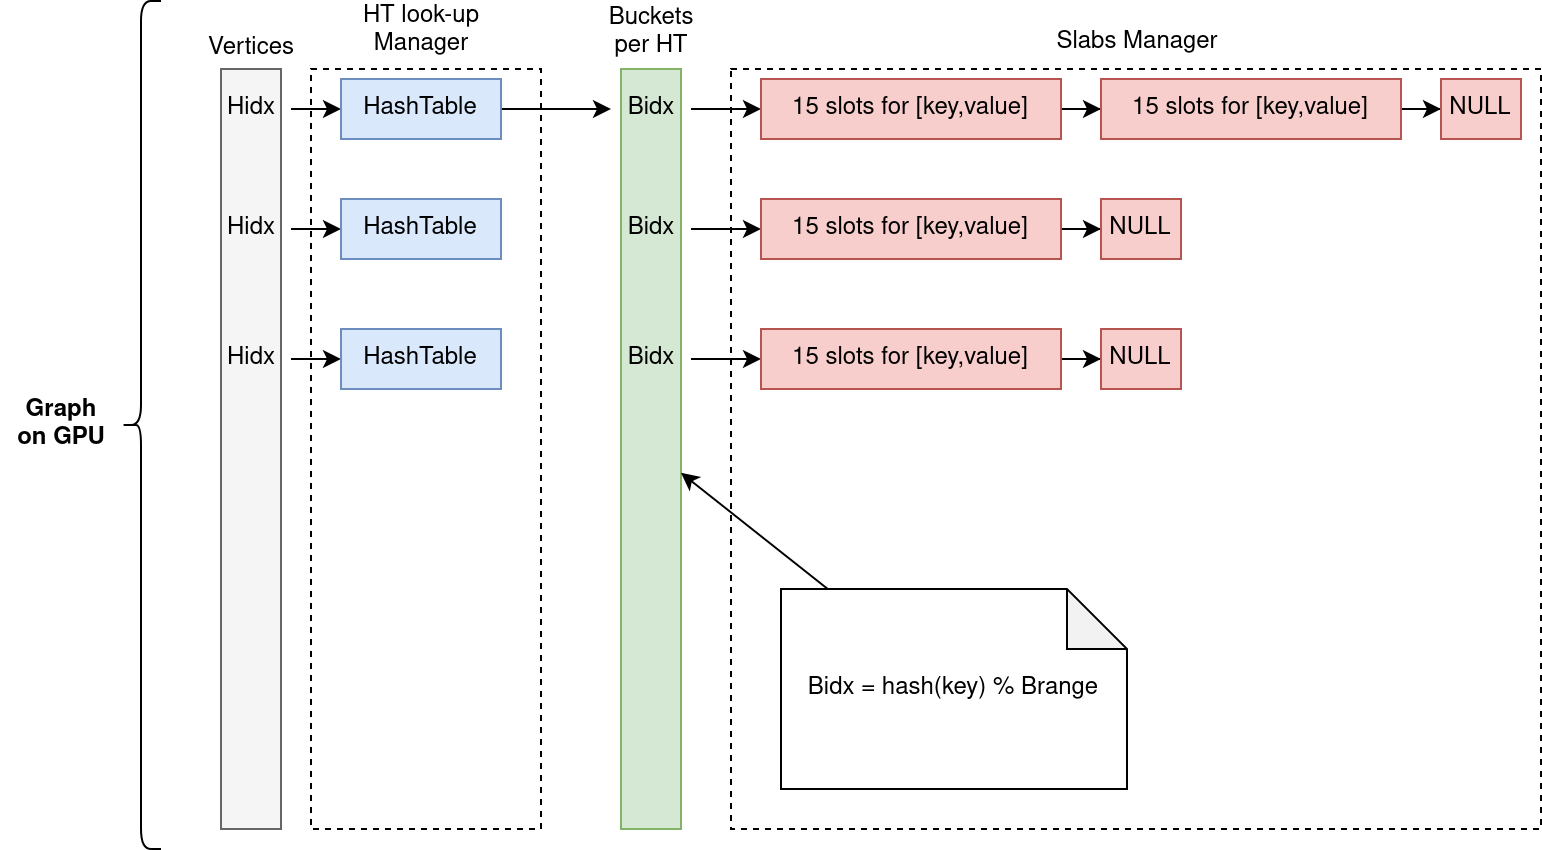
\includegraphics[width=\textwidth]{pictures/graph_gpu.png}
            \caption{Graph Structure on the GPU}
            \label{fig:graph_strucutre}
        \end{figure}
    \end{minipage}\hfill
\end{frame}

\begin{frame}[fragile] \frametitle{Операции над графом}
    \begin{itemize}
        \item Добавление ребра $(u,v,w)$
        \item Удаление ребра $(u,v)$
        \item Добавление вершины $u$
        \item Удаление вершины $u$
        \item Поиск ребра вида $(u,v)$
        \item \textbf{В данной реализации дублирование ребер с разными весами запрещено: при вставке ребра, если до этого существовало такое-же ребро, но с другим весом, то оно будет заменено}
    \end{itemize}
\end{frame}

\begin{frame}[fragile] \frametitle{Реализация}
    \begin{itemize}
        \item Как это устроено?
        \item Warp Cooperative Work Sharing (WCWS)
        \item GPU Slab Hash Table\footnote{A Dynamic Hash Table for the GPU, Saman Ashkiani, Martin Farach-Colton, John D. Owens, ссылка: \href{https://arxiv.org/abs/1710.11246}{https://arxiv.org/abs/1710.11246}}
    \end{itemize}
\end{frame}

\begin{frame}[fragile] \frametitle{WCWS: Идея}
    \begin{itemize}
        \item GPU состоит из стриминговых мульти-процессоров (SMs)
        \item В каждом таком SM фиксированное количество потоков, которые сгруппированы в SIMD блоки размером 32 потока, называемые warp 
        \item Каждый такой warp может исполнять только один \textbf{путь} программы на своих потоках
        \item Сильное ветвление $\implies$ замедление warp до 32 раз
        \item Решение: писать программу таким образом, что на warp почти всегда будет один путь ветвления, но на 32 вариациях данных
    \end{itemize}
\end{frame}

\begin{frame}[fragile] \frametitle{WCWS: Реализация}
    \begin{itemize}
        \item Каждый поток внутри warp имеет свою задачу
        \item Пока у потоков есть задачи:
        {
        \begin{itemize}
            \item \textit{Голосуют}, чья задача выполняется раньше
            \item Получают все одну задачу
            \item Читают непрерывный блок памяти, кратный 32
            \item Определяют свой статус
            \item Выбирают того, кто преуспел. Тот, кто преуспел, записывает результат
            \item Если никто не преуспел, переходят к следующему блоку памяти, иначе - задача решена
        \end{itemize}
        }
    \end{itemize}
\end{frame}

\begin{frame}[fragile] \frametitle{GPU Slab Hash Table}
    \begin{itemize}
        \item Разрешение коллизий - метод цепочек
        \item В качестве узлов - блоки памяти на 128 байт
        \item Один узел вмещает M = 15 пар (key,value), 4 байта на вспомогательную информацию, и 4 байта на индекс следующего узла в списке
        \item Максимальная эффективности по памяти $94\%$
        \item Среднее количество узлов в цепочке $\beta = \lceil N \ (M * B) \rceil$
        \item Эффективность по памяти: $\frac{N * x}{(M * x + y) * \Sigma k_i} \leq \frac{M * x}{M * x + y}$, где $x$ - размер пары, $y$ - размер индекса следующего узла, $k_i$ - длина $i$-ой цепочки
    \end{itemize}
\end{frame}

\begin{frame}[fragile] \frametitle{GPU Slab Hash Table}
    \begin{minipage}[m]{0.95\linewidth}
        \begin{figure}
            \centering
            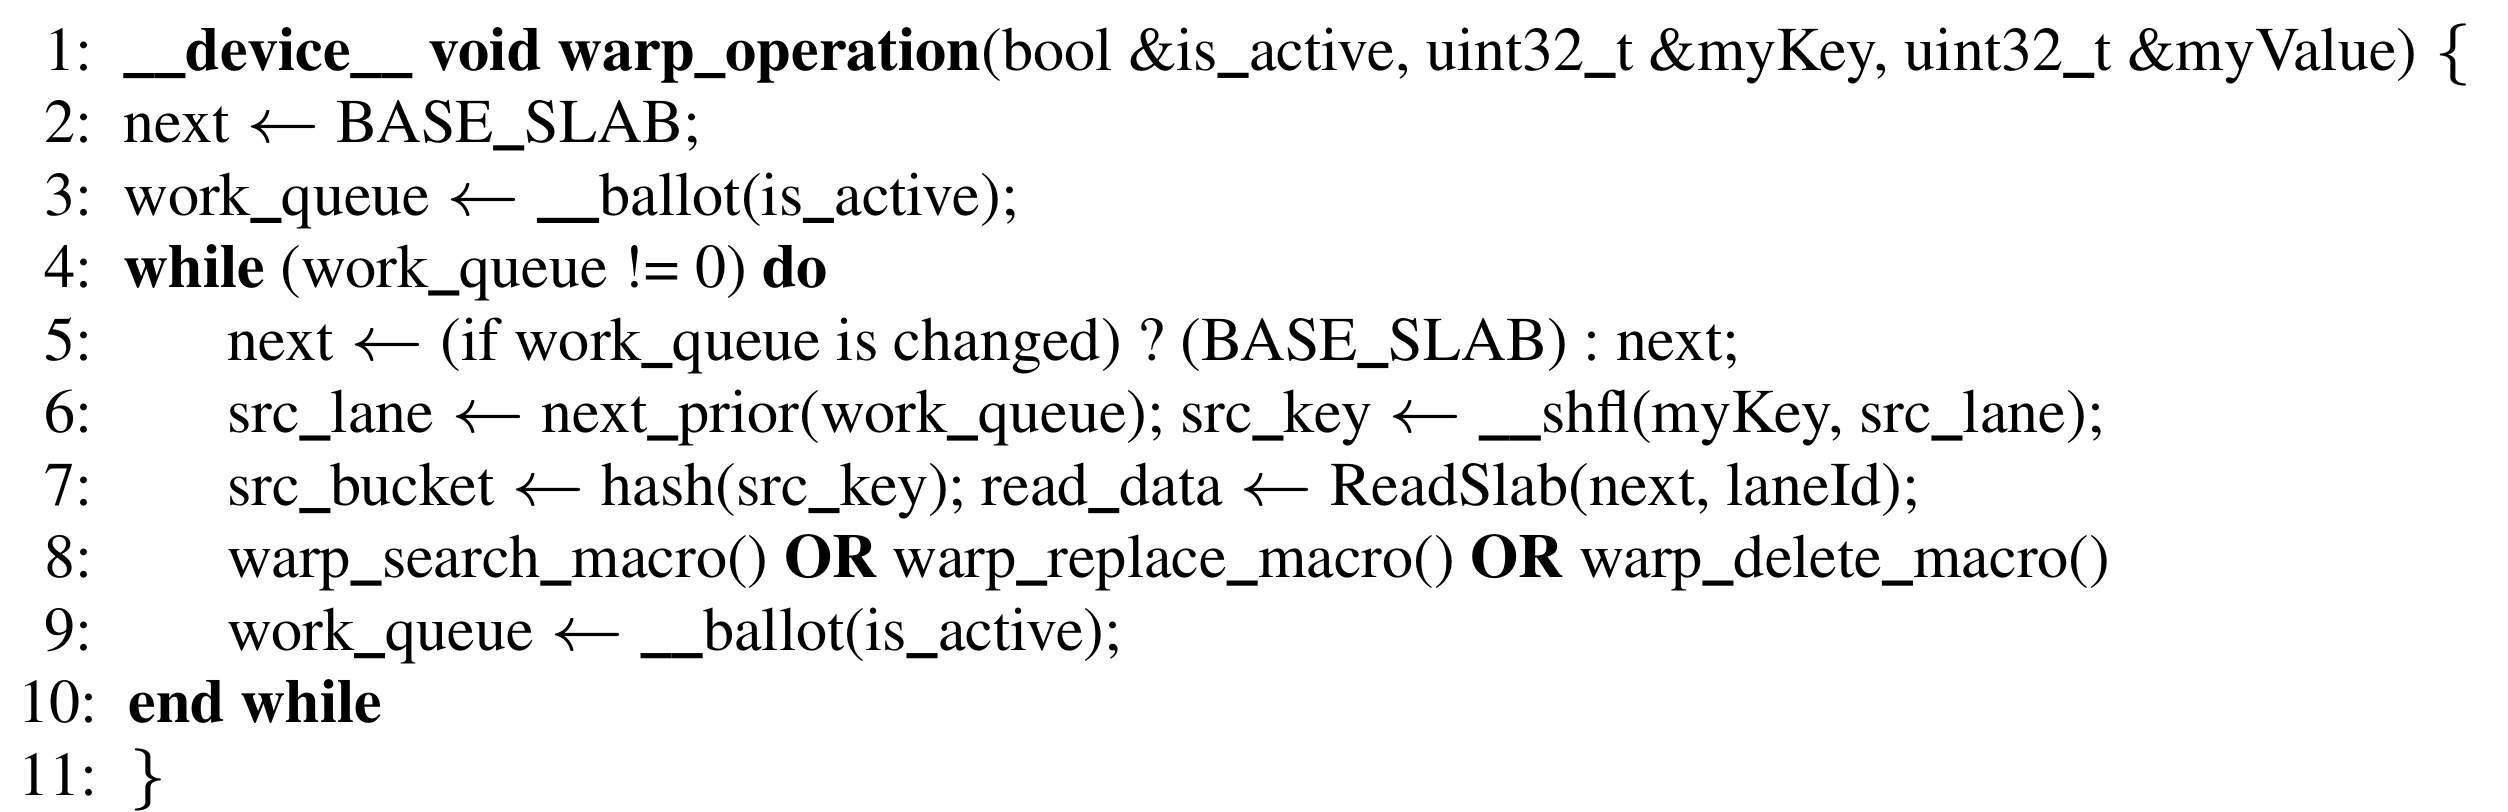
\includegraphics[width=\textwidth]{pictures/hashtable_pseudocode.png}
            \caption{Slab Hash Table Algo Pseudocode}
            \label{fig:pseudocode}
        \end{figure}
    \end{minipage}\hfill
\end{frame}

\begin{frame}[fragile] \frametitle{GPU Slab Hash Table}
    \begin{minipage}[m]{0.95\linewidth}
        \begin{figure}
            \centering
            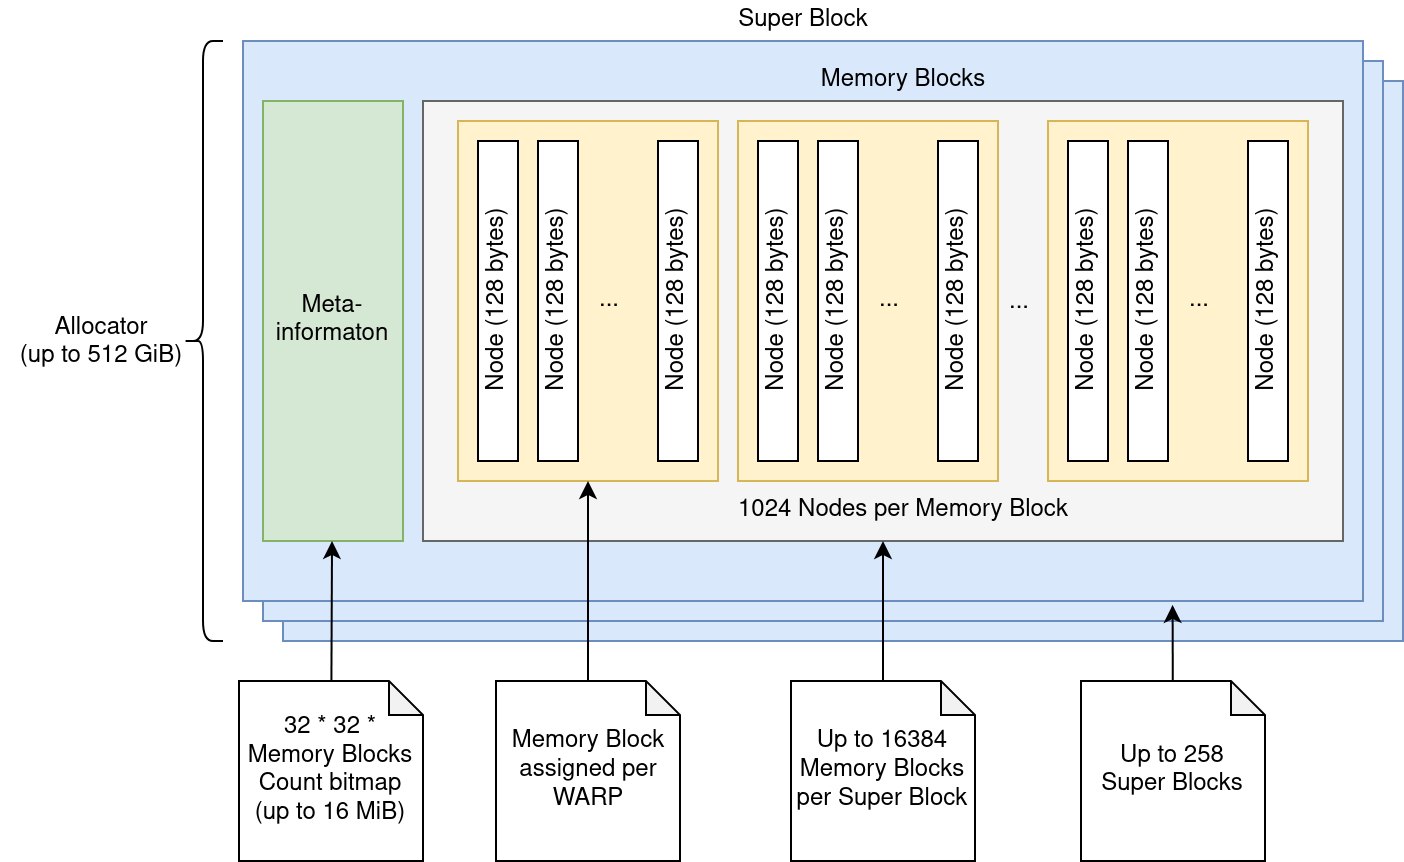
\includegraphics[width=\textwidth]{pictures/memory_allocator.png}
            \caption{VRAM Memory Allocator for Slab Hash Table}
            \label{fig:memory_allocator}
        \end{figure}
    \end{minipage}\hfill
\end{frame}

\begin{frame}[fragile] \frametitle{Динамические графы на GPU: Реализация}
    \begin{itemize}
        \item Помним про WCWS стратегию
        \item Вставка/удаление ребер:
        {
            \begin{itemize}
                \item Очередь ребер на warp
                \item Выбираем ребра с одинаковым src голосованием
                \item Получаем $src$ вершину
                \item $table \gets graph[src]$
                \item $table.replace(dst,weight)$ или $table.delete(dst)$
                \item Уменьшаем или увеличиваем число вершин, смежных с $src$
            \end{itemize}
        }
    \end{itemize}
\end{frame}

\begin{frame}[fragile] \frametitle{Динамические графы на GPU: Реализация}
    \begin{itemize}
        \item Удаление вершин немного сложнее:
        {
            \begin{itemize}
                \item Очередь вершин на warp
                \item Выбираем вершину голосованием
                \item Итерируемся по ее ребрам
                \item Для каждой такой $dst$ вершины исходящего ребра
                \item $table \gets graph[dst]$
                \item $table.delete(src)$
                \item Освобождаем память при необходимости
            \end{itemize}
        }
    \end{itemize}
\end{frame}

\begin{frame}[fragile] \frametitle{Динамические графы на GPU: Датасет}
    \begin{minipage}[m]{0.95\linewidth}
        \begin{figure}
            \centering
            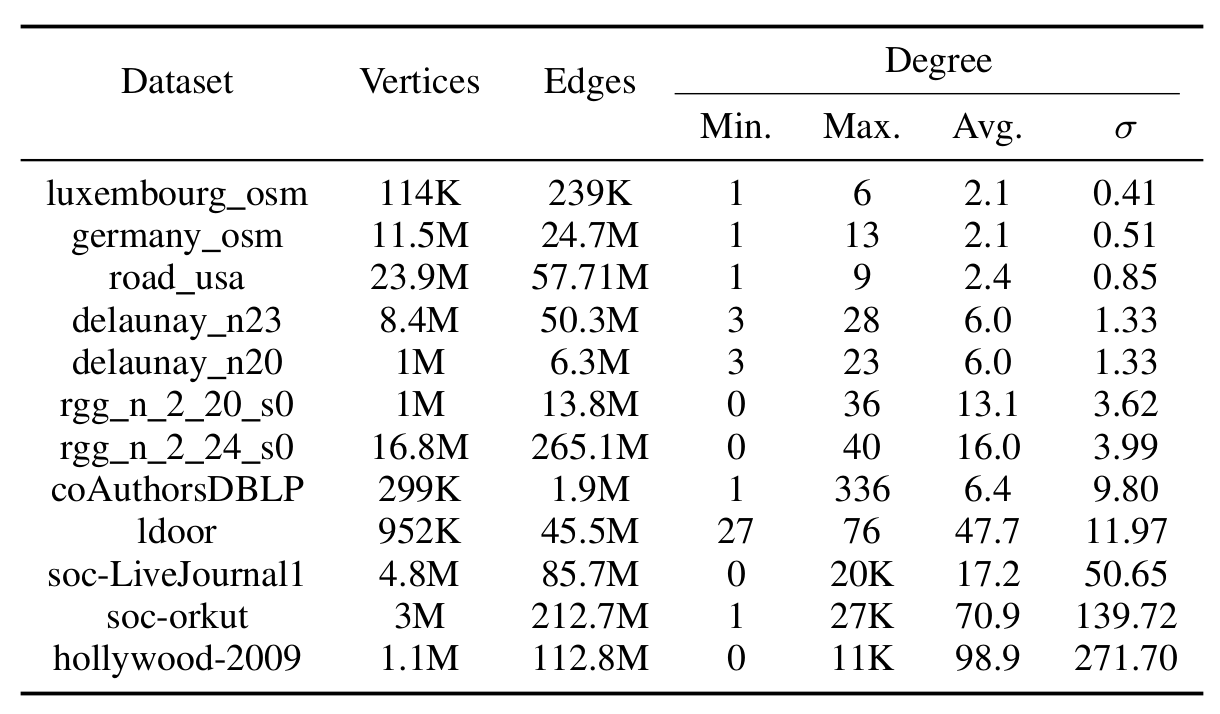
\includegraphics[width=\textwidth]{pictures/dataset.png}
            \caption{Graphs Datasets}
            \label{fig:dataset}
        \end{figure}
    \end{minipage}\hfill
\end{frame}

\begin{frame}[fragile] \frametitle{Динамические графы на GPU: Замеры}
    \begin{minipage}[m]{1.0\linewidth}
        \begin{figure}
            \centering
            \begin{subfigure}[b]{0.47\textwidth}
                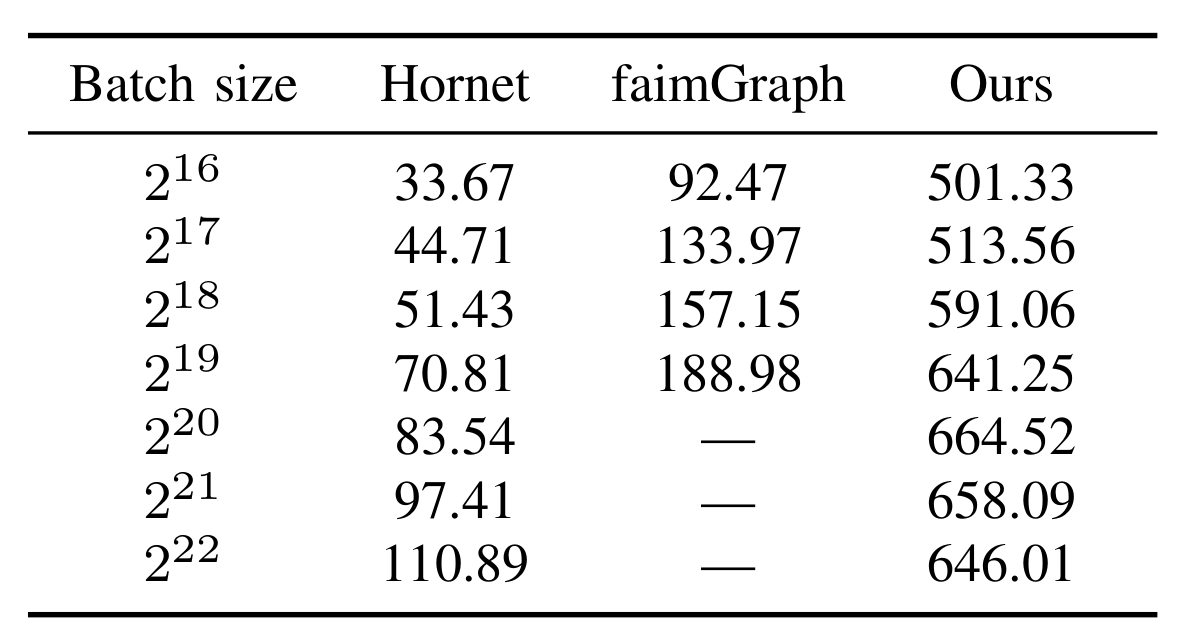
\includegraphics[width=\textwidth]{pictures/insertions.png}
                \caption{Insertions}
            \end{subfigure}
            \hfill
            \begin{subfigure}[b]{0.47\textwidth}
                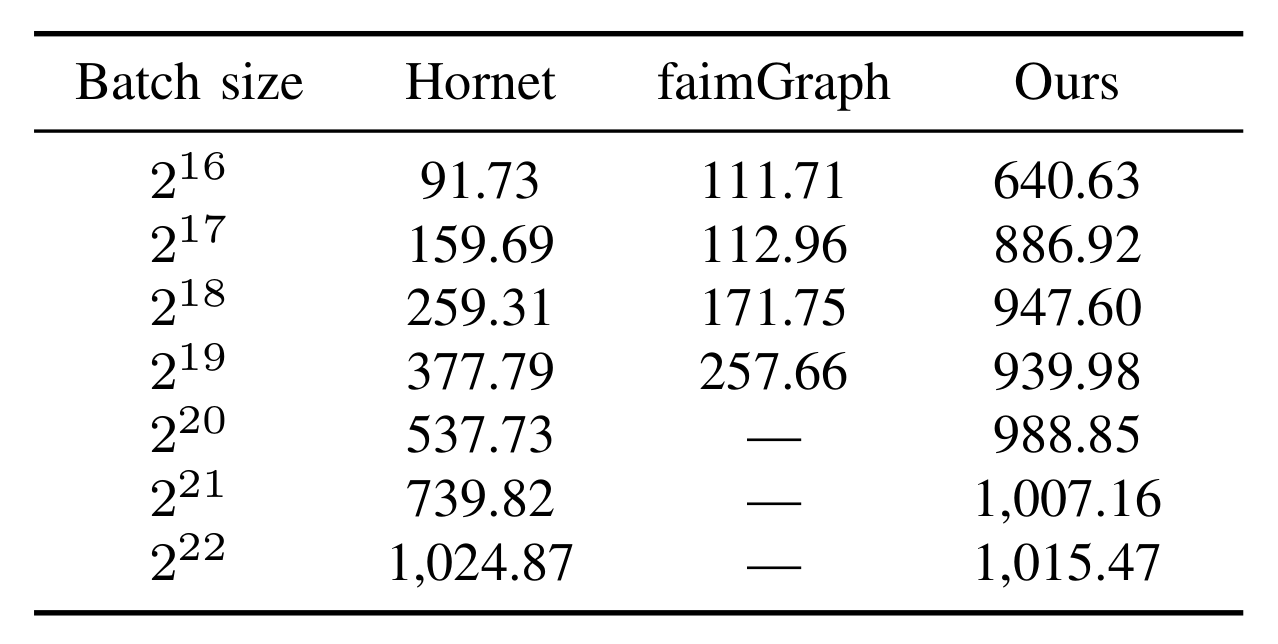
\includegraphics[width=\textwidth]{pictures/deletions.png}
                \caption{Deletions}
            \end{subfigure}
            \caption{Edge operations rate in MEdges/s}
        \end{figure}
    \end{minipage}\hfill
\end{frame}

\begin{frame}[fragile] \frametitle{Динамические графы на GPU: Замеры}
    \begin{minipage}[m]{1.0\linewidth}
        \begin{figure}
            \centering
            \begin{subfigure}[b]{0.47\textwidth}
                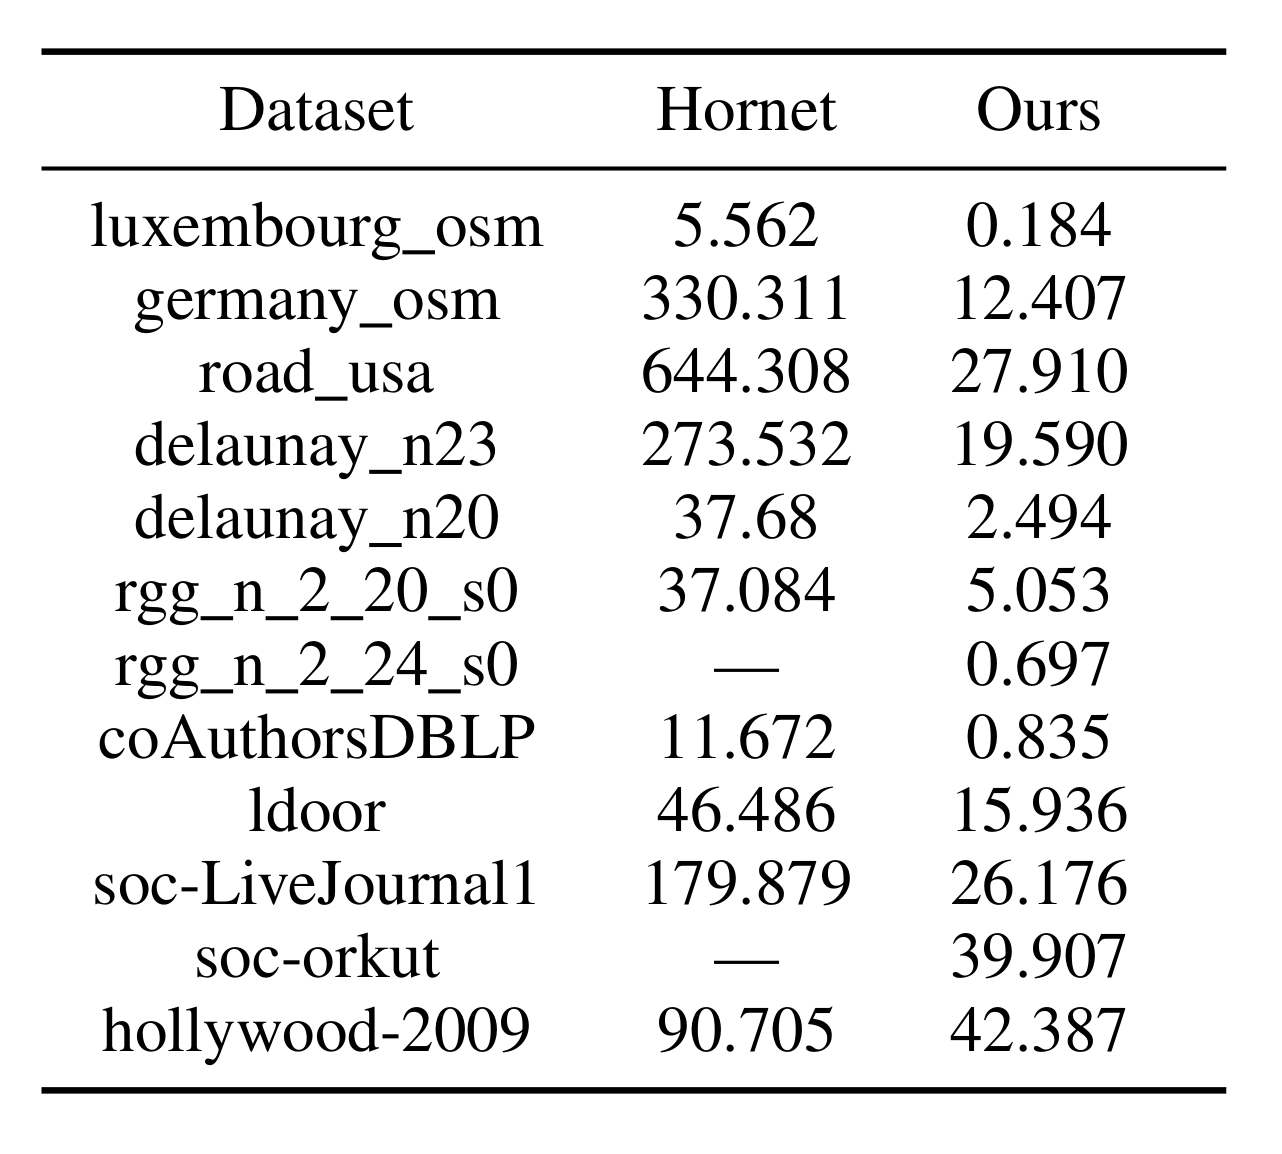
\includegraphics[width=\textwidth]{pictures/bulk_build.png}
                \caption{Bulk}
            \end{subfigure}
            \hfill
            \begin{subfigure}[b]{0.47\textwidth}
                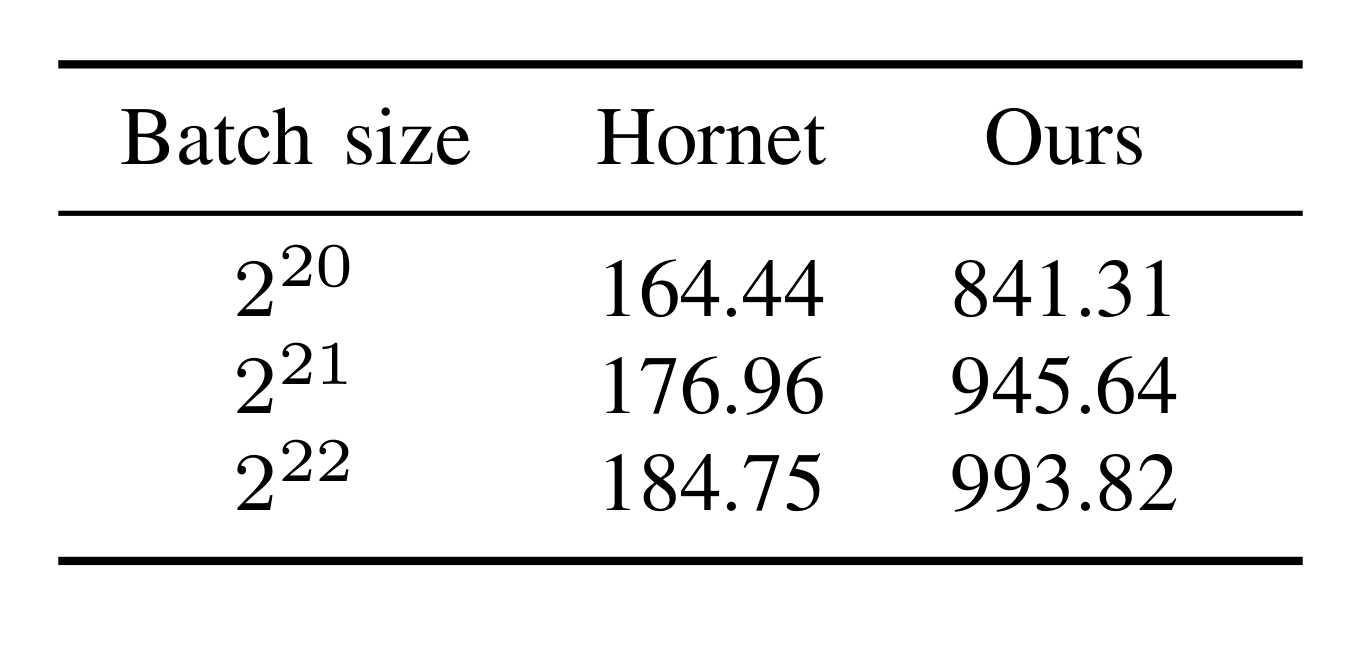
\includegraphics[width=\textwidth]{pictures/incremental_build.png}
                \caption{Incremental}
            \end{subfigure}
            \caption{Graph building}
        \end{figure}
    \end{minipage}\hfill
\end{frame}

\begin{frame}[fragile] \frametitle{Динамические графы на GPU: Замеры}
    \begin{minipage}[m]{0.95\linewidth}
        \begin{figure}
            \centering
            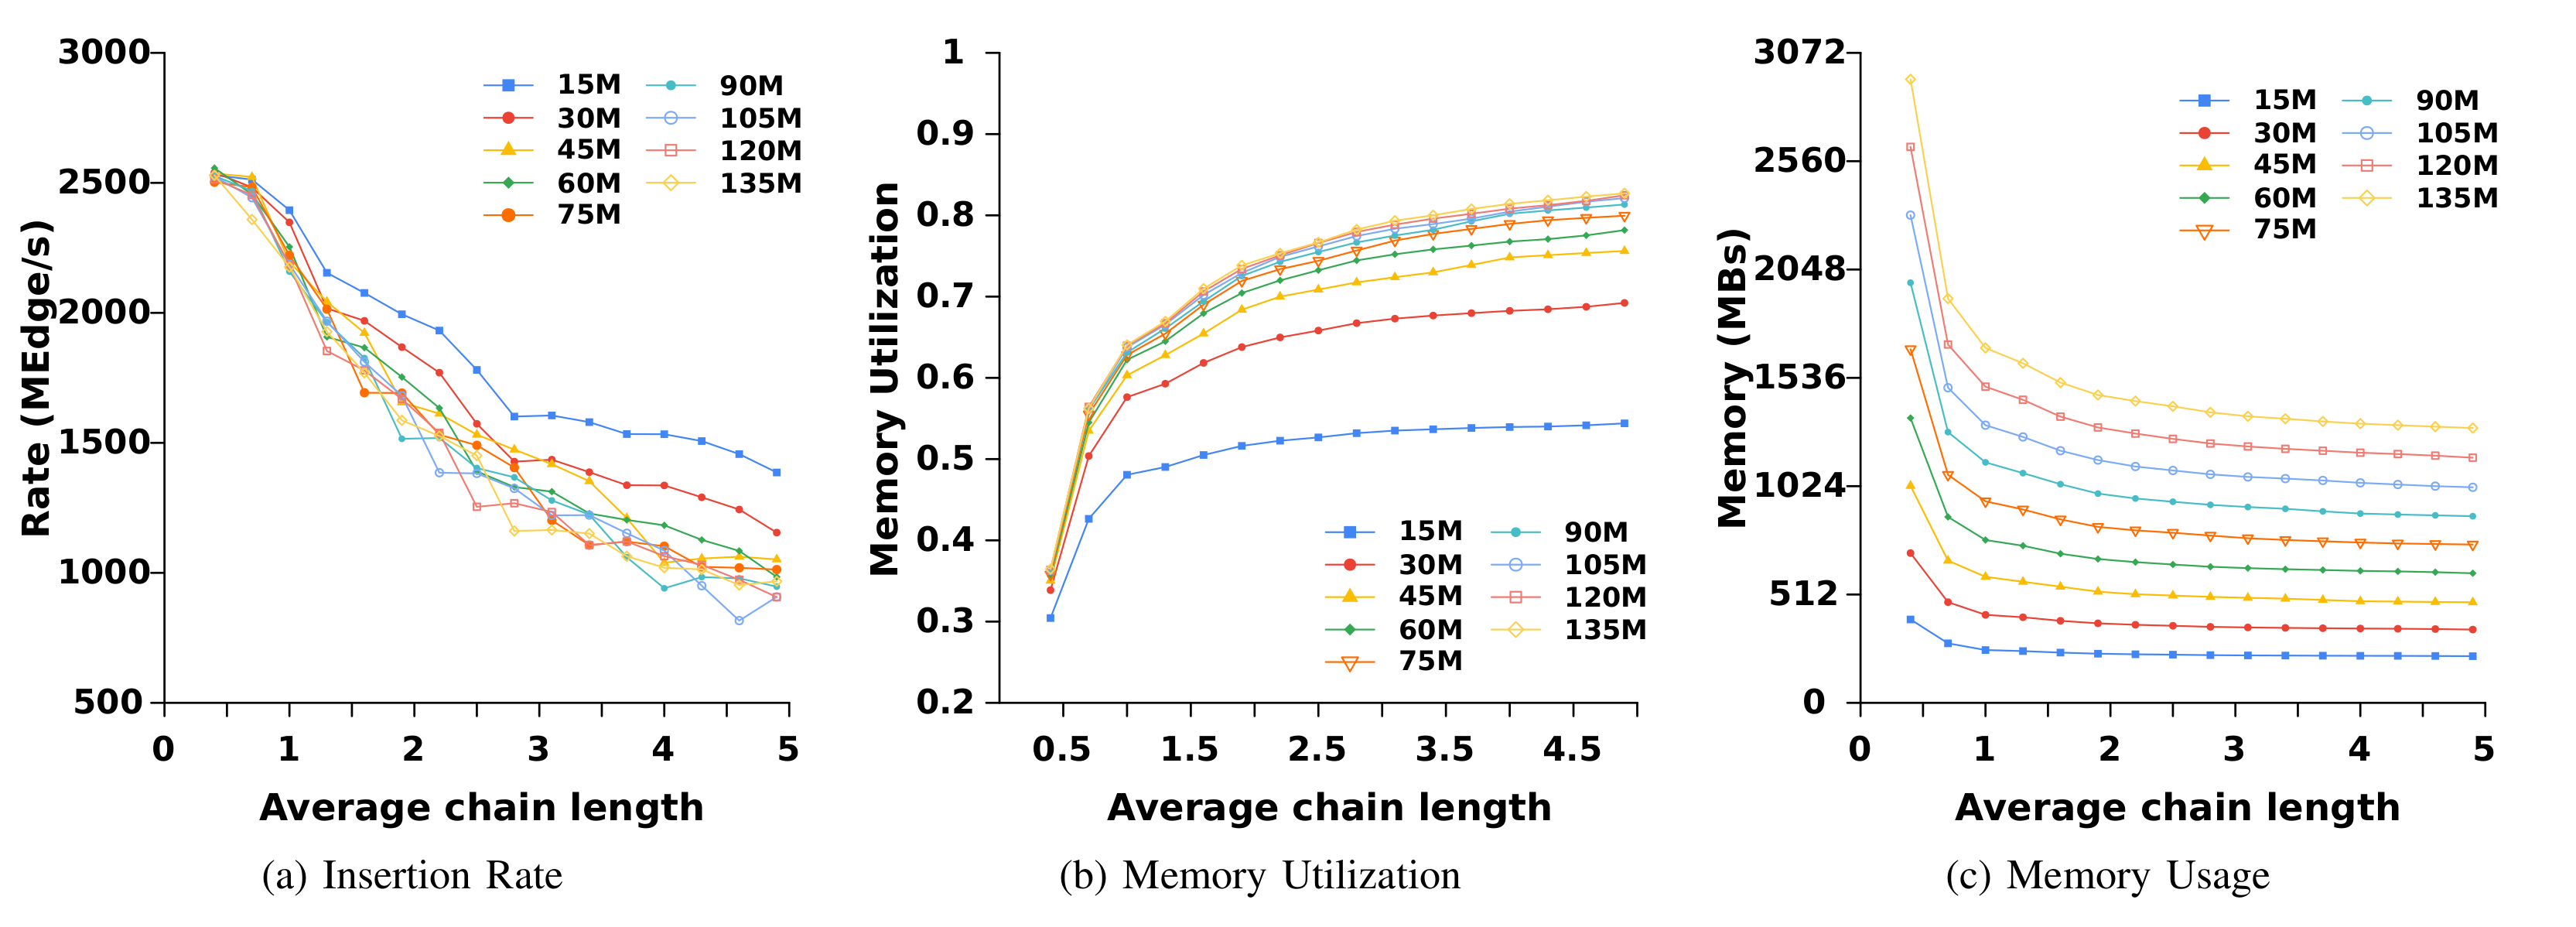
\includegraphics[width=\textwidth]{pictures/loadfactor.png}
            \caption{Loadfactor scalability}
            \label{fig:ld}
        \end{figure}
    \end{minipage}\hfill
\end{frame}

\begin{frame}[fragile] \frametitle{Итоги}
    \begin{itemize}
        \item Операции группируются \textit{per-batch}
        \item Только одна метка на ребро
        \item Скорость vs. Количество расходуемой памяти
        \item Хороший пример того, как использовать WCWS
        \item Решит ли unified-memory все проблемы?
    \end{itemize}
\end{frame}

\begin{frame} \frametitle{Дополнительно}
    \begin{itemize}
        \item Почта: \href{mailto:egororachyov@gmail.com}{egororachyov@gmail.com}
        \item Материалы презентации:
        {
            \begin{itemize}
                \item {Dynamic Graphs on the GPU, Muhammad A. Awad, 
              Saman Ashkiani, Serban D. Porumbescu et al., ссылка: 
              \href{https://escholarship.org/uc/item/48j4k7np}{https://escholarship.org/uc/item/48j4k7np}} 
                \item {A Dynamic Hash Table for the GPU, Saman Ashkiani, Martin Farach-Colton, John D. Owens, ссылка: \href{https://arxiv.org/abs/1710.11246}{https://arxiv.org/abs/1710.11246}}
            \end{itemize}
        }
    \end{itemize}
\end{frame}

\end{document}
